\chapter{SystemNaim: Implementation}

In its current implementation SystemNaim is able to generate a 2-FPGA system, with one parent and one child FPGA. \autoref{fig:indepth_full_sys} shows an in-depth view of the signals between every module in a multi-FPGA system. This diagram can be used as a reference by the reader, as we explore the implementation of each aspect of the system.

\begin{sidewaysfigure}
    \centering
    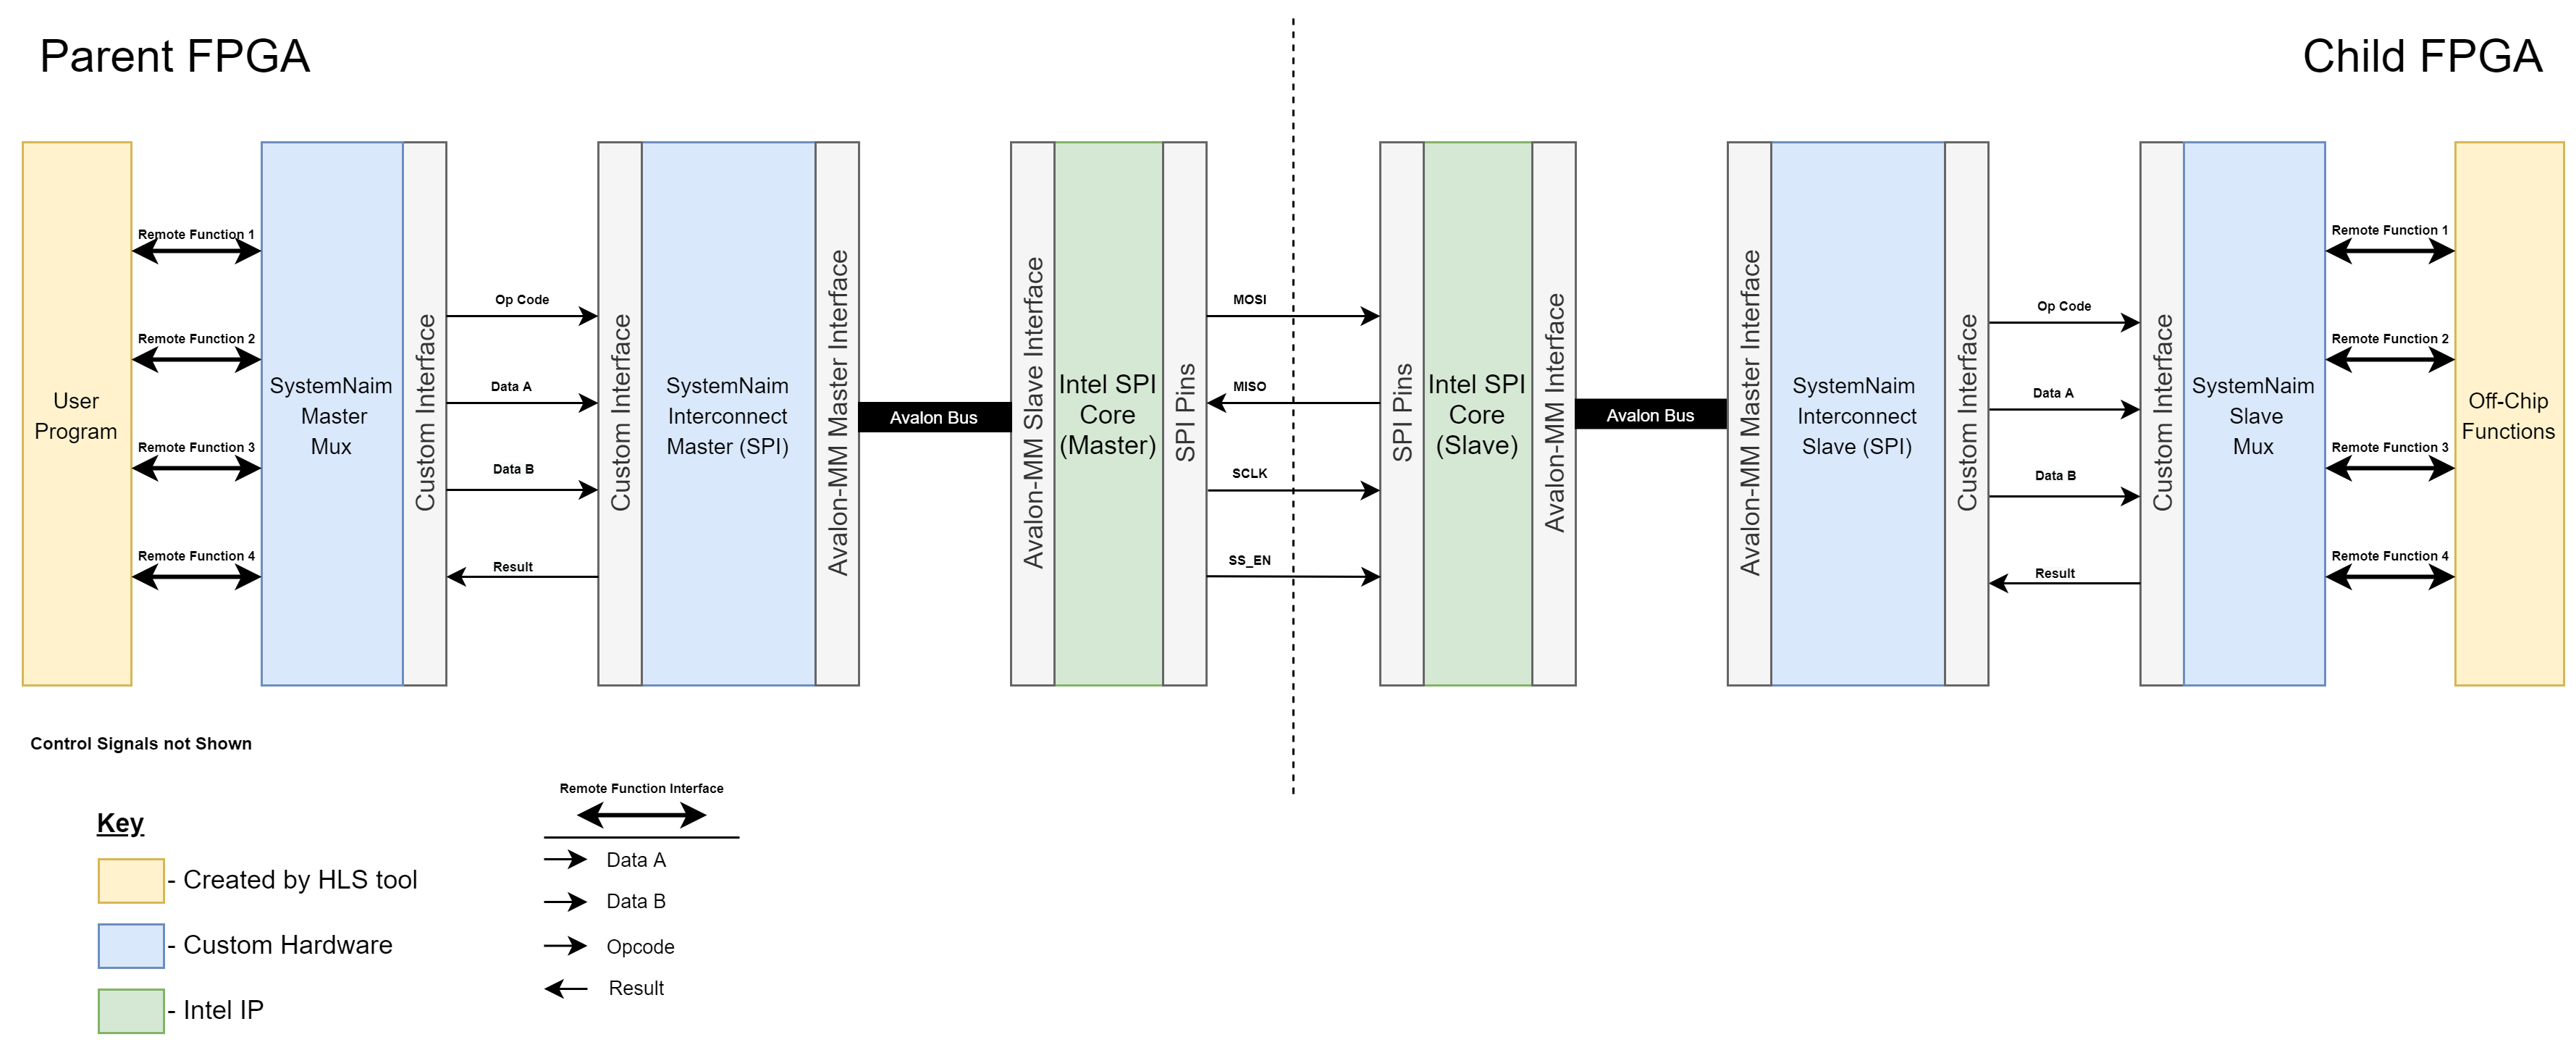
\includegraphics[width=\textwidth]{04_Implementation/images/FGPA_Interface_block_diagram.png}
    \caption{Full multi-FPGA system generated by SystemNaim, with signal names}
    \label{fig:indepth_full_sys}
\end{sidewaysfigure}


\section{HLS}
\label{sec:hls_impl}

The HLS part of SystemNaim is an ANSI C90 transpiler which targets Verilog. Since the focus of this investigation is not to create a fully features HLS tool, certain limitations have been placed on this aspect to reduce development time.

\begin{itemize}
    \item \textbf{The input will be a single source file}. Multiple files require pre-processing and linking to be implemented and offer only convenience to the user.
    \item \textbf{Only integer types will be allowed}. There is little difference between types in hardware except for the width of data, and thus a system that works with 32-bit values would likely work with 16-bit values, with the exception being floating point numbers. Regardless, having multiple types in a program makes very little difference when considering how it well it would perform on a multi-FPGA system and adding multiple types to the HLS would also require the addition of type checking. Thus, only 32-bit integers are allowed.
    \item \textbf{No arrays are allowed}. While many programs use arrays, they are not necessary for the purposes of this investigation. Since we are trying to show that automating the creation of a multi-FPGA system is possible, without the addition of too much latency, we can emulate programs which would iterate over array by simply creating a for loop. The array accesses themselves aren't of much interest to us, and thus the HLS tool has no need to implement them. This limitation also means we no longer have to deal with side effects that occur in most parallel programs, since there is no shared state/memory.
\end{itemize}

As for the method by which we transpile, we have opted to go for a line-to-state methodology, where every line of code translates to a set of states in Verilog. When the program is fully transpiled, the resulting Verilog will be an FSM which sequentially goes through all the states created from the code until it reaches the end. Loops and If Statements will break the sequential nature of the FSM but allowing them to jump to predefined states was a straightforward implementation.

Functions are implemented as their own Verilog modules. Each function call is equivalent to a module instantiation in Verilog, with the parent module being able to start the instantiated module at the appropriate time and then wait until the done signal is asserted, after which it can continue normal operation.

Each module implements a NIOS custom instruction interface \cite{nios-ii-inst-guide} at the top level which allows for control over the module. A breakdown of this interface is shown in \autoref{fig:nios_instr}. This will also be used to run the user program in a NIOS II system.

To further explain the implementation of the line-to-code methodology, we will go through a series of standard programming constructs which would be used in most user programs, as well as the two new constructs which have been added.

\begin{figure}[!htb]
    \centering
    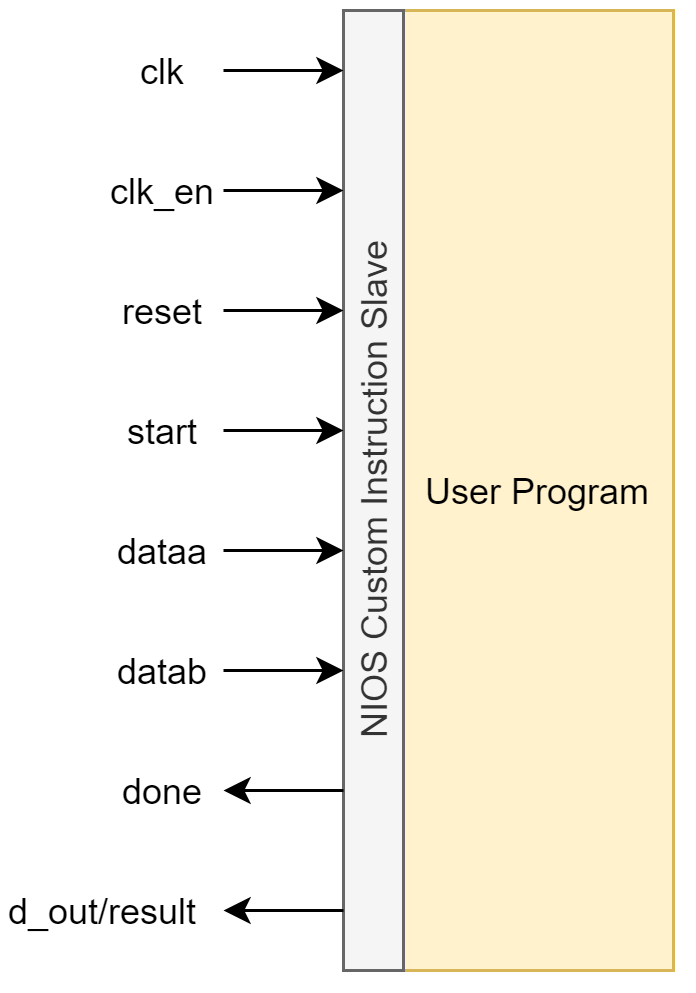
\includegraphics[width=0.4\textwidth]{04_Implementation/images/custom_instr_interface.png}
    \caption{NIOS custom instruction slave interface}
    \label{fig:nios_instr}
\end{figure}

\subsection{Variables}
\label{sn:var_sections}

Each variable in the user program is converted to two registers in the output HDL, as shown \autoref{sn:var}. The $var$\_next register is used in the combinational logic of the hardware if the value of $var$ needs to be changed, and at every positive edge of the clock cycle the $var$ register is set to the value $var$\_next register, \autoref{sn:var_update}. The $var$ register itself is used in the combinational logic if the value of $var$ is needed, such as in an arithmetic operation.

The method of using a “next” register for assignments is a standard Verilog practice and ensures that we avoid cyclic combinational logic in the generated HDL. 

\begin{figure}[H]
\centering
\begin{subfigure}{0.15\textwidth}
    \centering
    \begin{minted}{c}
int x;
    \end{minted}
\end{subfigure}%
{\LARGE$\rightarrow$}%
\begin{subfigure}{0.3\textwidth}
    \begin{minted}{Verilog}
reg [31:0] x;
reg [31:0] x_next;
    \end{minted}
\end{subfigure}
\caption{Variable Instantiation: Variable converted by SystemNaim.}
\label{sn:var}
\end{figure}

\begin{figure}[H]
\centering
\begin{subfigure}{0.15\textwidth}
    \centering
    \begin{minted}{c}
int x;
    \end{minted}
\end{subfigure}%
{\LARGE$\rightarrow$}%
\begin{subfigure}{0.45\textwidth}
    \begin{minted}[breaklines]{Verilog}
always_ff @ (posedge clk or posedge reset) begin
if(reset) begin
    x <= 32'd0;
end
else if (!clk_en) begin
    x <= 32'd0;
end
else begin
    x <= x_next;
    // State logic below
end
    \end{minted}
\end{subfigure}
\caption{Variable Update: Variable converted by SystemNaim.}
\label{sn:var_update}
\end{figure}

\subsection{Expressions}

Expressions are minly limited to arithmetic operations such as addition, subtraction, multiplication and division. Each of these operations within an expression is implemented as one state, therefore in cases such as \autoref{sn:expr}, only a single state is generated. However, when we there are multiple operations in an expression, as shown in \autoref{sn:expr_brackets}, temporary variables are generated to store the value of the intermediate calculations before completing the final assignment.

\begin{figure}[H]
\centering
\begin{subfigure}{0.2\textwidth}
    \centering
    \begin{minted}{c}
x = a + b;
    \end{minted}
\end{subfigure}%
{\LARGE$\rightarrow$}%
\begin{subfigure}{0.3\textwidth}
    \begin{minted}{Verilog}
assignment1: begin
    x_next = a + b;
end
    \end{minted}
\end{subfigure}
\caption{Assignment expression converted by SystemNaim.}
\label{sn:expr}
\end{figure}

\begin{figure}[H]
\centering
\begin{subfigure}{0.35\textwidth}
    \centering
    \begin{minted}{c}
x = ((4 * a) + b) / 2;
    \end{minted}
\end{subfigure}%
{\LARGE$\rightarrow$}%
\begin{subfigure}{0.47\textwidth}
    \begin{minted}{Verilog}
addChildLeft1: begin
    addLeft1_next = 32'd4 * a;
end
divChildLeft2: begin
    divLeft0_next = addLeft1 + b;
end
assignment3: begin
    x_next = divLeft0 / 32'd2;
end
    \end{minted}
\end{subfigure}
\caption{Assignment expression, with multiple operations, converted by SystemNaim.}
\label{sn:expr_brackets}
\end{figure}


\subsection{For Loops}

For loops generate four states, not including the states generated by the code inside the loop. The first state handles the initializer expression of the “for loop”, in the example shown in \autoref{sn:for} this would be the “assignment1” state, which performs the expression $i = 0$. The second state,“forCondExpr2”, assigns the result of the loop condition to a temporary variable which is then checked in the third state, “forBranch3”.

In \autoref{sn:for_state}, we can see that when the program is in this state, the program will either stay in the loop, and go to the first state generated by the code within the loop, or exit the loop which results in the FSM jumping to state generated just after the “for loop”.

The final state, “assignment4”, handles the increment expression in the “for loop”, which in this case just increments $i$ by one. The state logic also jumps to second state so that the condition can be re-evaluated.

\begin{figure}[H]
\centering
\begin{subfigure}{0.42\textwidth}
    \centering
    \begin{minted}{c}
for(i = 0; i < 20; i = i + 1){
    // Some code
}
    \end{minted}
\end{subfigure}%
{\LARGE$\rightarrow$}%
\begin{subfigure}{0.5\textwidth}
    \begin{minted}{Verilog}
assignment1: begin
    i_next = 32'd0;
end
forCondExpr2: begin
    forCond1_next = i < 32'd20;
end
forBranch3: begin
;
end
// Start of Verilog code inside loop
// ...
// ...
// End of Verilog code inside loop
assignment4: begin
    i_next = i + 32'd1;
end
    \end{minted}
\end{subfigure}
\caption{Combinational Logic: For Loop converted by SystemNaim.}
\label{sn:for}
\end{figure}

\begin{figure}[H]
\centering
\begin{subfigure}{0.42\textwidth}
    \centering
    \begin{minted}{c}
for(i = 0; i < 20; i = i + 1){
    // Some code
}
    \end{minted}
\end{subfigure}%
{\LARGE$\rightarrow$}%
\begin{subfigure}{0.48\textwidth}
    \begin{minted}[breaklines]{Verilog}
assignment1: begin
    state <= forCondExpr2;
end
forCondExpr2: begin
    state <= forBranch3;
end
forBranch3: begin
    state <= forCond1 ? /*Stay*/ : /*Exit*/;
end
// Start of code inside loop
// ...
// ...
// End of code inside loop
assignment4: begin
    state <= forCondExpr2;
end
\end{minted}
\end{subfigure}
\caption{State Logic: For Loop converted by SystemNaim.}
\label{sn:for_state}
\end{figure}

\subsection{If Statement}

An “if statement” in SystemNaim generates 2 states which are similar to the second and third state for a “for loop”. The first evaluates the condition, the second then jumps to the appropriate state. In the case of \autoref{sn:if_state}, if “cond0” was true the FSM would jump to the state which computed $y = 2$, whereas if the condition was false, it would instead compute $y = 3$. It should be noted that the code generated inside the true branch of the “if statement” does jump to the state generated after the “if statement” once its branch has finished processing, essentially the resulting hardware does exit the loop after the true branch has finished computation.

\begin{figure}[H]
\centering
\begin{subfigure}{0.22\textwidth}
    \centering
    \begin{minted}{c}
if (x > 4){
    y = 2;
} else {
    y = 3;
}
\end{minted}
\end{subfigure}%
{\LARGE$\rightarrow$}%
\begin{subfigure}{0.45\textwidth}
    \begin{minted}{Verilog}
ifCondExpr1: begin
    cond0_next = x > 32'd4;
end
ifBranch3: begin
;
end
    \end{minted}
\end{subfigure}
\caption{Combinational Logic: If Statement converted by SystemNaim.}
\label{sn:if}
\end{figure}

\begin{figure}[H]
\centering
\begin{subfigure}{0.22\textwidth}
    \centering
    \begin{minted}{c}
if (x > 4){
    y  = 2;
} else {
    y = 3;
}
\end{minted}
\end{subfigure}%
{\LARGE$\rightarrow$}%
\begin{subfigure}{0.6\textwidth}
    \begin{minted}{Verilog}
ifCondExpr1: begin
    state <= ifBranch3;
end
ifBranch3: begin
    state <= cond0 ? /*True*/ : /*False*/;
end
    \end{minted}
\end{subfigure}
\caption{State Logic: If Statement converted by SystemNaim.}
\label{sn:if_state}
\end{figure}

\subsection{Function Calls}
\label{sn:func_sec}

Function calls need module instantiations and as such require extra HDL outside the state and combinational logic. \autoref{sn:func_call_mdl} shows an example instantiation in Verilog, the name of the module is the same as the function name, but the instance name is generated by the tool to allow for multiple instantiation of the same module. As can be seen the “done” and “d\_out” signals have generated wires so that the tool can read the values outputted by the module. The function arguments, “a” and “b”, the “start” port and an additional register to hold the result of the function, have generated varaibles which store each of these values to them. The variables follow the same rules specified in \autoref{sn:var_sections}.

Function calls also add 2 states to the FSM, a function call and a function wait state. As in \autoref{sn:func_call_comb}, when in the function call state, the start signal for the appropriate module is asserted and the registers, which are connected to the input argument ports, are set to the required values. In the function wait state, the parent module waits for the “done” signal to be asserted at which point it captures the data on the “d\_out” wire and stores it in a generated register. This register is then used for any assignments or expression the function call was a part of.

The state logic in \autoref{sn:func_call_state}, shows that when in the function wait state, the FSM waits for the “done” signal to be asserted so that it can move onto the next state, otherwise it stays in the same state.

\begin{figure}[H]
\centering
\begin{subfigure}{0.25\textwidth}
    \centering
    \begin{minted}{c}
x = func(3, 5);
\end{minted}
\end{subfigure}%
{\LARGE$\rightarrow$}%
\begin{subfigure}{0.4\textwidth}
    \begin{minted}{Verilog}
wire func_done0;
wire [31:0] func_out0;
func func0(
    .clk(clk),
    .clk_en(clk_en),
    .reset(reset),
    .a(a0),
    .b(b0),
    .start(func_start0),
    .done(func_done0),
    .d_out(func_out0)
);
    \end{minted}
\end{subfigure}
\caption{Module Instantiation: Function Call converted by SystemNaim}
\label{sn:func_call_mdl}
\end{figure}

\begin{figure}[H]
\centering
\begin{subfigure}{0.25\textwidth}
    \centering
    \begin{minted}{c}
x = func(3, 5);
\end{minted}
\end{subfigure}%
{\LARGE$\rightarrow$}%
\begin{subfigure}{0.55\textwidth}
    \begin{minted}[breaklines]{Verilog}
funcCall1: begin
    a0_next = 32'd3;
    b0_next = 32'd5;
    func_start0_next = 1'd1;
end
funcWait2: begin
    func_start0_next = 1'd0;
    func_outData1_next = func_done0 ? func_out0 : func_outData1;
end
assignment3: begin
	x_next = func_outData1;
end
    \end{minted}
\end{subfigure}
\caption{Combinational Logic: Function Call converted by SystemNaim}
\label{sn:func_call_comb}
\end{figure}

\begin{figure}[H]
\centering
\begin{subfigure}{0.25\textwidth}
    \centering
    \begin{minted}{c}
x = func(3, 5);
\end{minted}
\end{subfigure}%
{\LARGE$\rightarrow$}%
\begin{subfigure}{0.55\textwidth}
    \begin{minted}[breaklines]{Verilog}
funcCall1: begin
    state <= funcWait2;
end
funcWait2: begin
    state <= func_done0 ? assignment3 : state;
end
assignment3: begin
	state <= return5;
end
    \end{minted}
\end{subfigure}
\caption{State Logic: Function Call converted by SystemNaim}
\label{sn:func_call_state}
\end{figure}

\subsection{Multi-Function Calls}

We can now explain the implementation for the constructs not found in original C90 grammar. The first construct allows users to call functions in parallel, and has more restrictions than a normal function call. Firstly, all function calls that the user wished to run parallel must be contained within a “split” block, an example of which is shown in \autoref{sn:multi_func_call_mdl}. Each line in the “split” block must contain an assignment expression with only a function call on the right-hand side.

The module instantiation for each function call follows the layout outlined in \autoref{sn:func_sec}, however, there is another example here to show that even if two modules have the same argument names, different register and wire names are generated for each one.

The way in which the functions are called is also similar to the single function case, however, as shown in \autoref{sn:multi_func_call_state}, in the function call state, “splitCall2”, the start signals for both modules are asserted, and the input registers are set to the right value. You may notice that here we use another variable as an input argument, this is also possible for single function calls, we are just showcasing how it is implemented in this example. 

The major difference lies in the addition of the “done” register. This is due to the fact that done signals are only asserted for a single cycle, and thus we need a register to indicate if a module has completed execution in the past. Modules running in parallel may have different latencies so relying solely on the “done” wire would result in the FSM stalling in most cases. Once the “done” registers for every module are set to 1, the FSM can move onto the next state. The logic for this is shown in \autoref{sn:multi_func_call_state}.

Once all functions have finished execution, the assignments are then processed.

\begin{figure}[H]
\centering
\begin{subfigure}{0.32\textwidth}
    \centering
    \begin{minted}{c}
split{
    a = func_a(x, 5);
    b = func_b(y, 5);
}
\end{minted}
\end{subfigure}%
{\LARGE$\rightarrow$}%
\begin{subfigure}{0.45\textwidth}
    \begin{minted}[breaklines]{Verilog}
wire func_a_done0;
wire [31:0] func_a_out0;
func_a func_a0(
    .clk(clk),
    .clk_en(clk_en),
    .reset(reset),
    .a(a0),
    .b(b0),
    .start(func_a_start0),
    .done(func_a_done0),
    .d_out(func_a_out0)
);

wire func_b_done5;
wire [31:0] func_b_out5;
func_b func_b5(
    .clk(clk),
    .clk_en(clk_en),
    .reset(reset),
    .a(a5),
    .b(b5),
    .start(func_b_start5),
    .done(func_b_done5),
    .d_out(func_b_out5)
);
    \end{minted}
\end{subfigure}
\caption{Module Instantiation: Multi-Function Call converted by SystemNaim}
\label{sn:multi_func_call_mdl}
\end{figure}


\begin{figure}[H]
\centering
\begin{subfigure}{0.32\textwidth}
    \centering
    \begin{minted}{c}
split{
    a = func_a(x, 5);
    b = func_b(y, 5);
}
\end{minted}
\end{subfigure}%
{\LARGE$\rightarrow$}%
\begin{subfigure}{0.58\textwidth}
    \begin{minted}[breaklines]{Verilog}
splitCall2: begin
    a0_next = x;
    b0_next = 32'd5;
    func_a_start0_next = 1'd1;
    func_a_doneReg2_next = 1'd0;
    a5_next = y;
    b5_next = 32'd5;
    func_b_start5_next = 1'd1;
    func_b_doneReg7_next = 1'd0;
end
splitWait3: begin
    func_a_start0_next = 1'd0;
    func_a_outData1_next = func_a_done0 ? func_a_out0 : func_a_outData1;
    func_a_doneReg2_next = func_a_done0 ? 1'b1 : func_a_doneReg2;
    func_b_start5_next = 1'd0;
    func_b_outData6_next = func_b_done5 ? func_b_out5 : func_b_outData6;
    func_b_doneReg7_next = func_b_done5 ? 1'b1 : func_b_doneReg7;
end
funcReturn4: begin
    a_next = func_a_outData1;
end
funcReturn5: begin
    b_next = func_b_outData6;
end
    \end{minted}
\end{subfigure}
\caption{Combinational Logic: Multi-Function Call converted by SystemNaim}
\label{sn:multi_func_call_comb}
\end{figure}

\begin{figure}[H]
\centering
\begin{subfigure}{0.32\textwidth}
    \centering
    \begin{minted}{c}
split{
    a = func_a(h, n);
    b = func_b(h, n);
}
\end{minted}
\end{subfigure}%
{\LARGE$\rightarrow$}%
\begin{subfigure}{0.58\textwidth}
    \begin{minted}[breaklines]{Verilog}
splitCall2: begin
    state <= splitWait3;
end
splitWait3: begin
    state <= func_a_doneReg2 && func_b_doneReg7 ? funcReturn4 : state;
end
funcReturn4: begin
    state <= funcReturn5;
end
funcReturn5: begin
    state <= return6;
end
    \end{minted}
\end{subfigure}
\caption{State Logic: Multi-Function Call converted by SystemNaim}
\label{sn:multi_func_call_state}
\end{figure}

\subsection{Remote Function Call}


Finally, we can move onto the last construct we are going to discuss: the remote function call. The remote function call allows users to run hardware on the child FPGA in parallel with a function on the parent FPGA. This is done similarly to the multi-function call except the calls are contained within a “split\_fpga” block, like the code segment shown in \autoref{sn:rmt_func_call_mdl}. Currently, only two function calls can be placed inside a “split\_fpga” block, both must also be assignment expressions with a sole function call on the right-hand side. The first function call is the one that will be run off-chip. So in this example, “func\_a” would be placed on the child FPGA.

When a function is run off-chip, the system produces two top files, the “host\_top” for the parent FPGA and the “remote\_top” for the child FPGA. On the “host\_top” file, a different module is instantiated for the off-chip function which has the suffix “remote”(shown in \autoref{sn:rmt_func_call_mdl}). The module has the same inputs and outputs as the normal function module with the addition of signals which allow it to interface with the interconnect. The logic inside this module, instead of processing the function, initiates a remote function call by starting the interconnect module, this details of how a remote function call works will be explained later. Once the interconnect has been started the “remote\_module”, then waits for the “data\_from\_remote\_valid” signal to go high, at which point it grabs the data from the “data\_from\_remote" bus and then asserts it's “done” signal, passing the data it received to the parent module. This means the FSM doesn't distinguish between a function run on-chip and a function which has been run on the child FPGA.

In addition, to allow for multiple modules throughout the program to be run off-chip, a multiplexer is provided which is placed in-between the “remote\_modules” and the interconnect. Each module connects to its own set of ports on the multiplexer, as shown in \autoref{sn:rmt_func_call_mst_mux}, and when one of the “select\_in” signals is asserted, the multiplexer forwards to appropriate data to the interconnect. Once the interconnect returns data to the multiplexer, the multiplexer then passes the data back to the module whose “select\_in” signal was high. The value of the “opcode\_out” bus is dependent on which module initiated the multiplexer, if the module connected on the first set of ports asserted its “select\_in” then the opcode value would be 1. If the second module started the multiplexer then the value would be 2 and so on. This value is important as it's used by the hardware on the child FPGA to select which module to execute.

\begin{figure}[H]
\centering
\begin{subfigure}{0.32\textwidth}
    \centering
    \begin{minted}{c}
split_fpga{
    a = func_a(3, 5);
    b = func_b(3, 5);
}
\end{minted}
\end{subfigure}%
{\LARGE$\rightarrow$}%
\begin{subfigure}{0.58\textwidth}
    \begin{minted}[breaklines]{Verilog}
wire func_a_done0;
wire [31:0] func_a_out0;
wire func_a_start_out0;
wire [31:0] func_a_dataa0;
wire [31:0] func_a_datab0;
wire [31:0] func_a_return0;
wire func_a_returnValid0;

func_a_remote func_a0(
    .clk(clk),
    .clk_en(clk_en),
    .reset(reset),
    .a(a0),
    .b(b0),
    .start(func_a_start0),
    .done(func_a_done0),
    .d_out(func_a_out0),
    .select_out(func_a_start_out0),
    .dataa_out(func_a_dataa0),
    .datab_out(func_a_datab0),
    .data_from_remote(func_a_return0),
    .data_from_remote_valid (func_a_returnValid0)
);
    \end{minted}
\end{subfigure}
\caption{Module Instantiation: Remote Function Call converted by SystemNaim}
\label{sn:rmt_func_call_mdl}
\end{figure}

\begin{figure}[H]
\centering
\begin{subfigure}{0.32\textwidth}
    \centering
    \begin{minted}{c}
split_fpga{
    a = func_a(3, 5);
    b = func_b(3, 5);
}
\end{minted}
\end{subfigure}%
{\LARGE$\rightarrow$}%
\begin{subfigure}{0.58\textwidth}
    \begin{minted}[breaklines]{Verilog}
sysNaim_master_mux mux0(
    .clk(clk),
    .start_out(start_out),
    .opcode_out(opcode_out),
    .dataa_out(dataa_out),
    .datab_out(datab_out),
    .data_from_remote(data_from_remote),
    .data_from_remote_valid (data_from_remote_valid),

    .select_in1(func_a_start_out0),
    .dataa_in1(func_a_dataa0),
    .datab_in1(func_a_datab0),
    .data_from_remote_in1 (func_a_return0),
    .data_from_remote_valid_in1 (func_a_returnValid0),

    .select_in2(1'b0),
    .select_in3(1'b0),
    .select_in4(1'b0)
);
    \end{minted}
\end{subfigure}
\caption{SystemNaim Master Multiplexer: Remote Function Call converted by SystemNaim \\ \textit{Additional signals would be present if multiple functions were connected.}}
\label{sn:rmt_func_call_mst_mux}
\end{figure}

\subsubsection{Child FPGA Hardware}

Since a “remote\_top” module is now present, it is worth talking about the modules that have been instantiated in this file due to the remote function call. The slave interconnect is present alongside, a slave multiplexer which interfaces with the interconnect, and the module for the function that was called off-chip. In this case that would be “func\_a”.

Shown in \autoref{sn:rmt_func_call_slv_mdl}, the “func\_a” module here contains all the state and combinational logic to compute the “func\_a” function in code. This module is controlled by the slave multiplexer, shown in \autoref{sn:rmt_func_call_slv_mux}. When the multiplexer receives data from the slave interconnect it means a remote function call has begun, and depending on the opcode received from the interconnect, the multiplexer then asserts the appropriate “start\_out” signal in order to initiate the correct module. Once the module has finished computation, it passes the result back to the multiplexer, which then passes it back to the interconnect to be sent back across the channel to the parent FPGA.

\begin{figure}[H]
\centering
\begin{subfigure}{0.32\textwidth}
    \centering
    \begin{minted}{c}
split_fpga{
    a = func_a(3, 5);
    b = func_b(3, 5);
}
\end{minted}
\end{subfigure}%
{\LARGE$\rightarrow$}%
\begin{subfigure}{0.58\textwidth}
    \begin{minted}[breaklines]{Verilog}
sysNaim_slave_mux mux0(
    .clk(clk),
    .start_in(data_to_hls_valid),
    .opcode_in(opcode),
    .dataa_in(dataa),
    .datab_in(datab),
    .data_to_host(data_from_hls),
    .data_to_host_valid (data_from_hls_valid),

    .start_out1(start1),
    .dataa_out1(dataa1),
    .datab_out1(datab1),
    .data_from_remote1 (data_from_remote1),
    .data_from_remote_valid1 (data_from_remote_valid1)
);
    \end{minted}
\end{subfigure}
\caption{SystemNaim Slave Multiplexer: Remote Function Call converted by SystemNaim \\ \textit{This module is instantiated on the child FPGA. Additional signals would be present if multiple functions were connected.}}
\label{sn:rmt_func_call_slv_mux}
\end{figure}

\begin{figure}[H]
\centering
\begin{subfigure}{0.32\textwidth}
    \centering
    \begin{minted}{c}
split_fpga{
    a = func_a(3, 5);
    b = func_b(3, 5);
}
\end{minted}
\end{subfigure}%
{\LARGE$\rightarrow$}%
\begin{subfigure}{0.58\textwidth}
    \begin{minted}[breaklines]{Verilog}
func_a m1(
    .clk(clk),
    .clk_en(clk_en),
    .reset(reset),
    .start(start1),
    .done(data_from_remote_valid1),
    .d_out(data_from_remote1),
    .a(dataa1),
    .b(datab1)
);
    \end{minted}
\end{subfigure}
\caption{Remote Module Instantiation: Remote Function Call converted by SystemNaim \\ \textit{This module is instantiated on the child FPGA}}
\label{sn:rmt_func_call_slv_mdl}
\end{figure}
        
    

\section{Interconnect}
\label{sec:impl_interconnect}

There are two interconnects in a multi-FPGA system generated by SystemNaim: the master interconnect, which is found on the parent FPGA, and the slave interconnect, which is found on the child FPGA. The responsibility of the master interconnect is to accept transactions from the master multiplexer, and send these transactions across the communication channel to the slave interconnect. The slave interconnect is designed to wait until it receives a transaction from the channel, at which point it passes this transaction onto the slave multiplexer which then initiates the off-chip function call.

Once the off-chip function call is complete, the return data is given to the slave interconnect by the slave multiplexer, which then transmits the data back across the communication channel. The master interconnect, at this point, will have been waiting for some valid return data on the communication and once it receives the valid data it passes to the master multiplexer, thus completing the job of the interconnect.

Each of these interconnects contains 2 sub-modules which allows for more modularity in the system, and each will be explored further in the following sections.

\subsection{Master Interconnect}

Shown in \autoref{fig:master_interconnect}, the master interconnect consists of 2 sub-modules: the “instruction encoder” and the “SPI Master Handler”. The former is exposed to the master multiplexer while the latter connects to the Intel SPI Core(Master), which controls the communication channel. When the “encoder” receives a transaction, by the multiplexer asserting the “start” signal, it checks to see if the “ready” signal has been asserted by the “handler”, if so it then sequentially sends the values from the: “opcode”, “dataa” and “datab” busses across the “data” bus between itself and the “handler”. Once all three values have been sent over, the “encoder” asserts the “start\_return” signal which indicates to the “handler” to start waiting for valid data to be returned on the communication channel. When the “return\_valid” signal is asserted by the “handler”, the “encoder” then passes the data back to the multiplexer.

The “SPI master handler” is designed to specifically interface the Intel SPI Core so that it can control the channel. It must first instruct the SPI core to transmit the data values passed to it by the “encoder”. Once the “start\_return” signal is asserted, the “handler” tells the SPI core to continuously poll for valid data from the child FPGA. The reason the master SPI core has to keeping polling the slave core is because the slave on an SPI channel cannot initiate transactions. When any transaction is started by the master SPI core on the parent FPGA, the slave SPI core starts simultaneously transmitting data stored in an internal register. At some point during operation, this internal register will contain the result of the off-chip function call, but that point cannot be determined beforehand and thus arises the need for continuous polling transactions, a diagram of this process is shown in \autoref{fig:interconnect_polling}.

The “handler” knows when valid data has been returned from the child FPGA if the most significant bit of the data it received was set to 1, this does limit the size of the return data to 31 bits, however, most programs are unaffected by the limitation. Once it does detect valid data, it passes it back to the “encoder” by asserting the “return\_valid” signal, and presenting the data, without the MSB set to 1, on the “return\_data” bus. 

\begin{figure}[!htbtb]
    \centering
    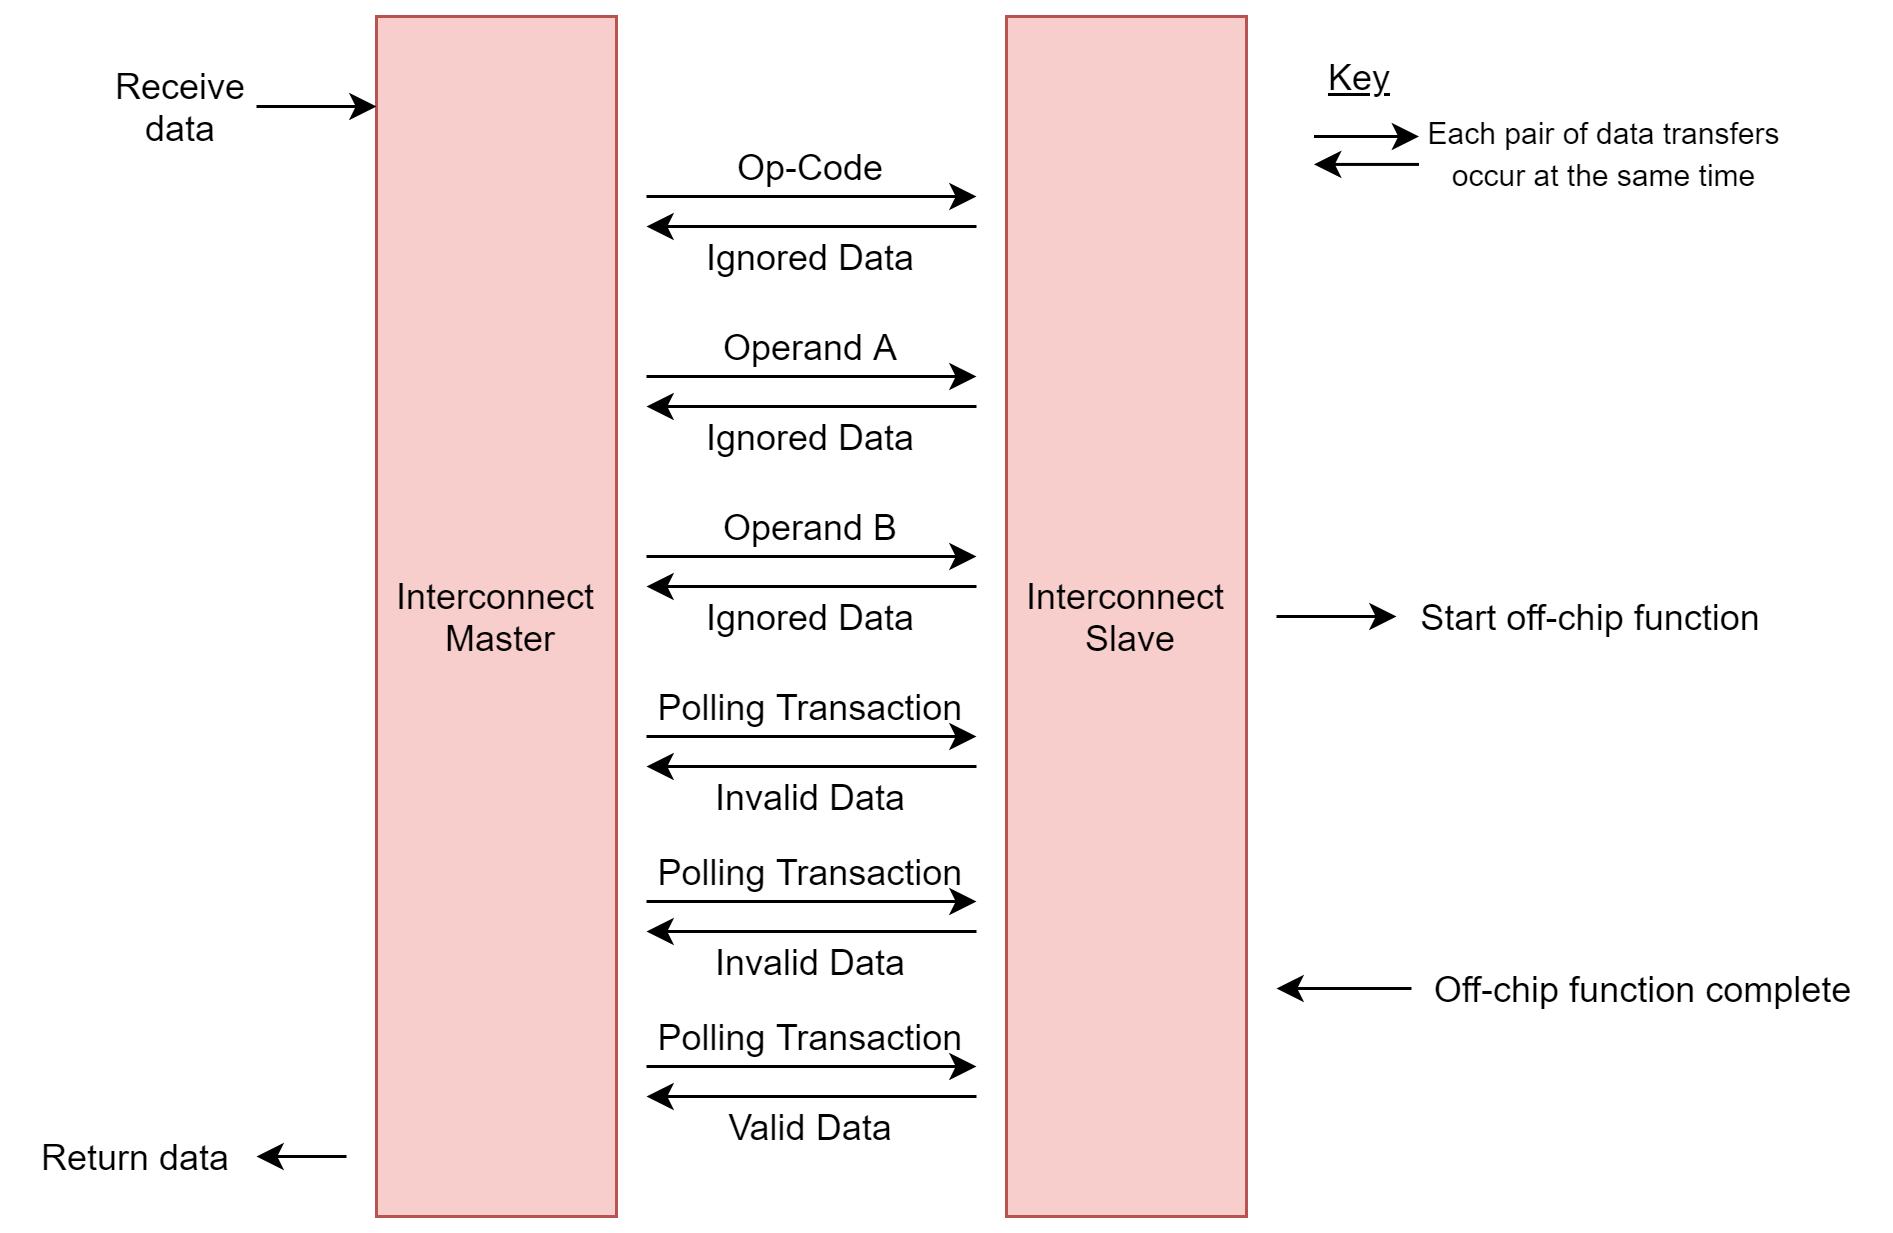
\includegraphics[width=0.9\textwidth]{05_evaluation/images/interconnect_polling.png}
    \caption{Example of interconnect communication protocol in practice}
    \label{fig:interconnect_polling}
\end{figure}


\begin{figure}[!htb]
    \centering
    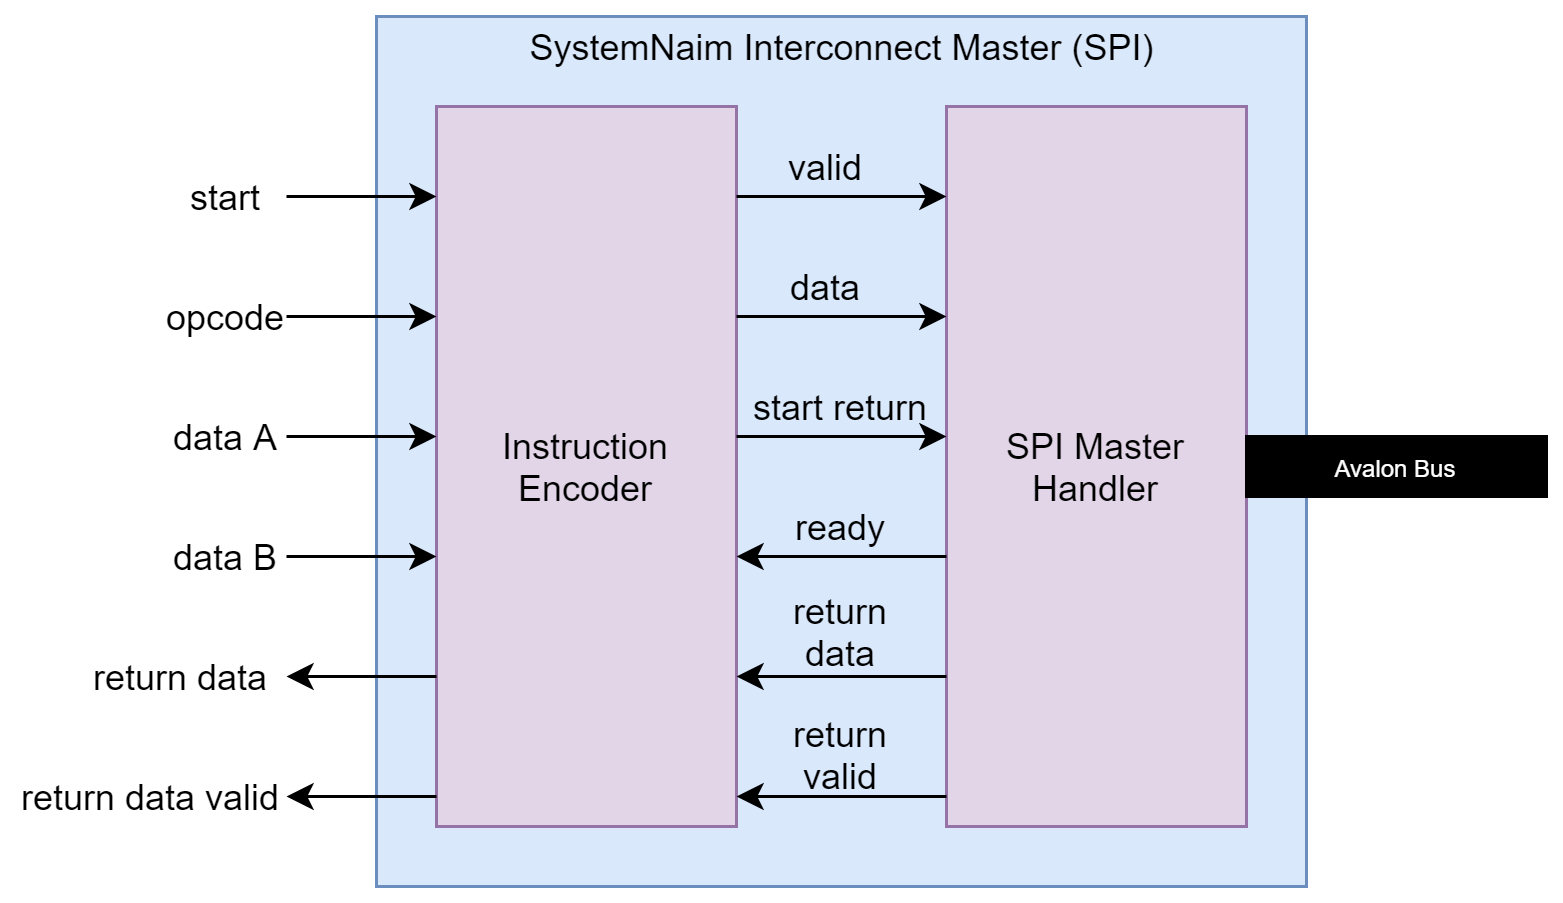
\includegraphics[width=0.9\textwidth]{04_Implementation/images/interconnect_block_diagram.png}
    \caption{Block diagram of the SystemNaim master interconnect.}
    \label{fig:master_interconnect}
\end{figure}

\subsection{Slave Interconnect}

The slave interconnect performs a similar job to the master interconnect but with the roles slightly reversed. As show in \autoref{fig:slave_interconnect}, the slave interconnect contains an “SPI Slave Handler” and an “Instruction Decoder”, where the former connect to an Intel SPI Core(Slave) and the latter is connected to the slave multiplexer. In this interconnect, the “handler” keeps checking the SPI core to see if it has received any data, if it has it then passes the data to the “decoder”. The “decoder” waits for data to be passed to it from the “handler”, and once it has received values for the: “opcode”, “dataa” and “datab”, it asserts “start\_return”, to tell the “handler” to now wait until the “decoder” provides valid return data from the off-chip function. The “decoder” then passes the received values to the slave multiplexer and waits until it is given some return data.

Once the off-chip function is complete and the multiplexer has passed the data back to the “decoder”, the “decoder” then passes the data to the “handler”. The “handler” gives the data, with the MSB set to 1 to indicate valid data, to the Slave SPI Core which is then stored in its internal register waiting for the parent FPGA to initiate a transaction. Thus, completing the role of the slave interconnect in the process of an off-chip function call.

\begin{figure}[!htb]
    \centering
    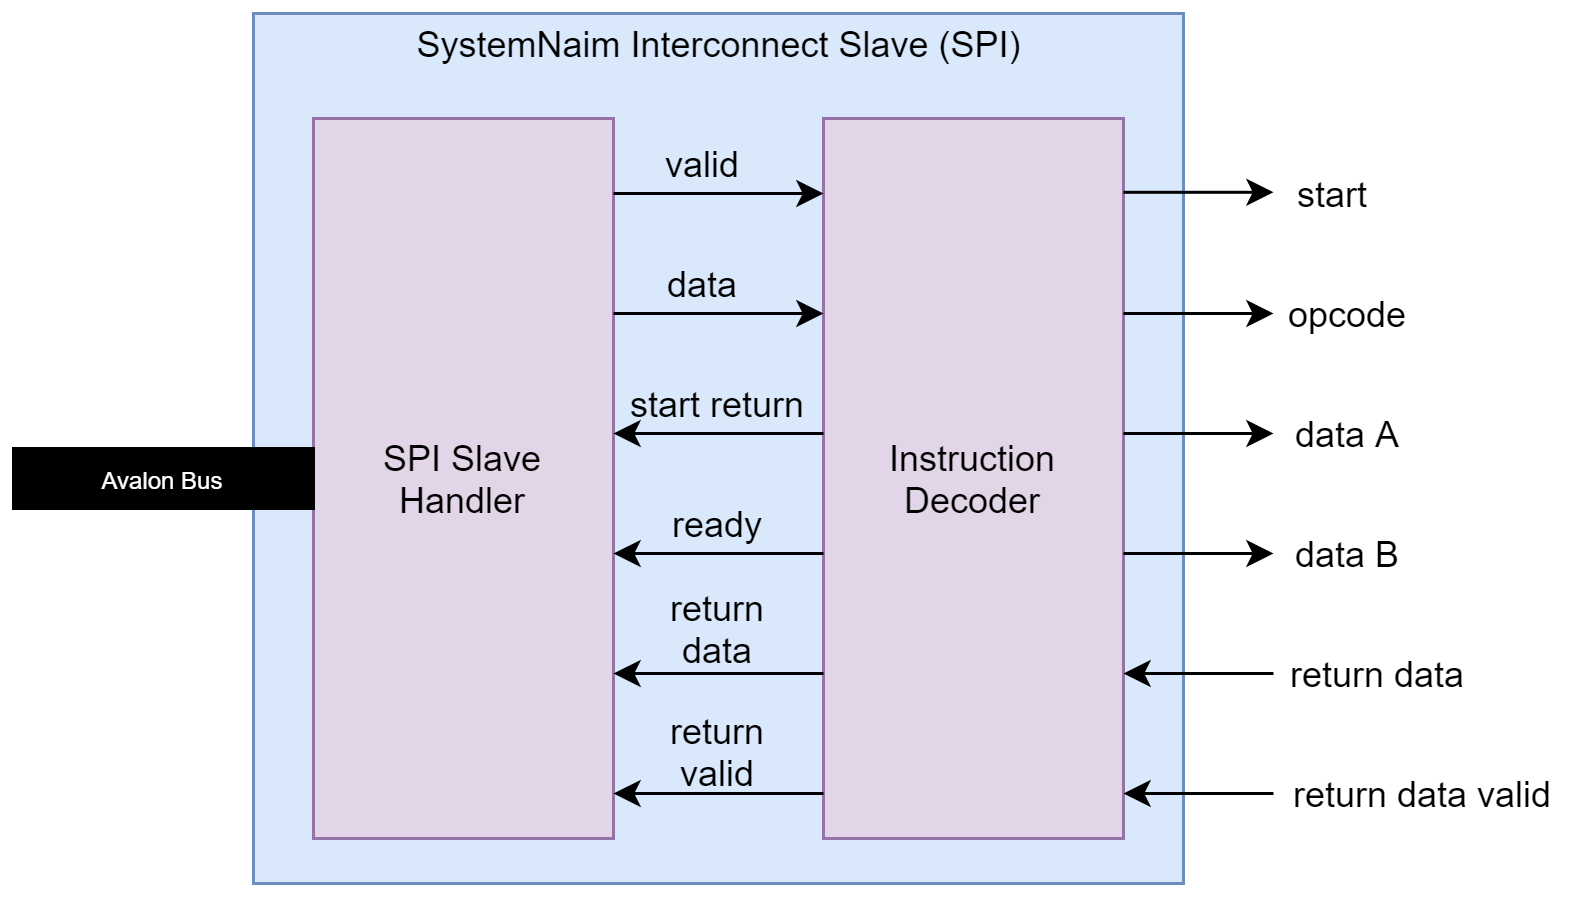
\includegraphics[width=0.9\textwidth]{04_Implementation/images/interconnect_slave.png}
    \caption{Block diagram of the SystemNaim slave interconnect.}
    \label{fig:slave_interconnect}
\end{figure}

\subsection{Modularity}

It has been mentioned in \autoref{sec:interconnect_design} that the design of the interconnect was performed with modularity in mind. This is achieved in implementation through the splitting of the interconnect into the two aforementioned modules. If, for example, we wanted to use an Ethernet channel instead of an SPI channel, the entirety of SystemNaim does not need to be re-written, nor even a large part of it. Instead, we simply need new “handler” modules for both the master and slave interconnect. These new modules would need to implement the same interface that connects with the “encoder” or “decoder”, but beyond that, the rest of the system would remain untouched. 

The same is possible for the “encoder” module, so that it can interface with a different HLS tool, or hardware system, but this would require the new system to follow the protocol specified by the “encoder” which may be more difficult.

In summary, the implementation of the interconnect is how we fulfil the modularity requirement specified in \autoref{sec:interconnect_design}, and allow users to choose the best communication protocol available to them.

\section{Communication Channel}

For the communication channel it was decided that the SPI communication protocol would be used due to its ease of implementation. SPI may not perform very well, but we can very easily account for the latency its adds to the total system and extrapolate about how using a faster protocol would affect the system. As mentioned in the design section, we just needed to be able to get the two FPGAs to communicate with each other.

The communication channel was not directly controlled by custom hardware. Instead, we opted to use Intel's SPI Core which was able to control the pins of the SPI Channel: MISO, MOSI, S\_CLK and SS\_EN, once given instructions through an Avalon-MM interface. Further information can be found in chapter 5 of \cite{intel-embedded-periph}. Most other communication protocols have similar IP core's made available by Intel, and thus all that would be required to use them would be new master and slave handler modules in both interconnects.